\documentclass{article}

\usepackage{xstring}
\usepackage{calc}
\usepackage{xintexpr}
\usepackage{arrayjobx}
\usepackage{tikz}
\usetikzlibrary{matrix}
\usepackage{etoolbox}

\newcommand\imgwidth{25}
\newcommand\imgheight{6}
\newcommand\pixelcount{0}

\renewcommand\pixelcount{\the\numexpr \imgwidth * \imgheight}

\typeout{moin}

\newread\file
\openin\file=input.txt
\read\file to \input % Reads a line of the file into \input  
\closein\file 

\typeout{Loaded file}

\newcommand\inputone{\input}
\newcommand\inputtwo{\input}

\newarray\bitmap
\expandarrayelementtrue

\newcommand\updatelayer[1]{
    \foreach \i in {1,...,\pixelcount}{
        \StrMid{#1}{\i}{\i}[\char]
        \IfEq{\char}{0}{
            \updatearray{\i}{0}
        }{
            \IfEq{\char}{1}{
                \updatearray{\i}{1}
            }{
                \IfEq{\char}{2}{
                    \updatearray{\i}{2}
                }{}
            }
        }
    }
}

\newcommand\updatearray[2]{
    \checkbitmap(#1)
    \ifemptydata
        \bitmap(#1)={#2}
    \else
        \if 2\cachedata \bitmap(#1)={#2} \fi
    \fi
}



\newcount\minzero
\minzero=\pixelcount
\newcount\onetimestwo
\newcount\ones
\newcount\twos

\newcount\counter
\counter=0
\loop
    \typeout{\the\counter}
    \StrLeft{\inputone}{\pixelcount}[\layer]
    \StrGobbleLeft{\inputone}{\pixelcount}[\inputone]
    \StrLen{\layer}[\layerlength]
    \ifnum \layerlength=\pixelcount
        \updatelayer{\layer}
        \StrCount{\layer}{0}[\zerocount]
        \ifnum \zerocount<\minzero
            \StrCount{\layer}{1}[\onecount]
            \StrCount{\layer}{2}[\twocount]
            \minzero=\zerocount
            \ones=\onecount
            \twos=\twocount
            \onetimestwo=\the\numexpr \onecount * \twocount \relax
        \fi
    \fi
    \advance \counter \pixelcount
\ifx\inputone\empty
\else
\repeat

\begin{document}

\section{Part 1}

Zeros: \the\minzero

$1*2$: \the\onetimestwo

Ones: \the\ones

Twos: \the\twos

\section{Part 2}

% 0: black
% 1: white
% 2: transparent

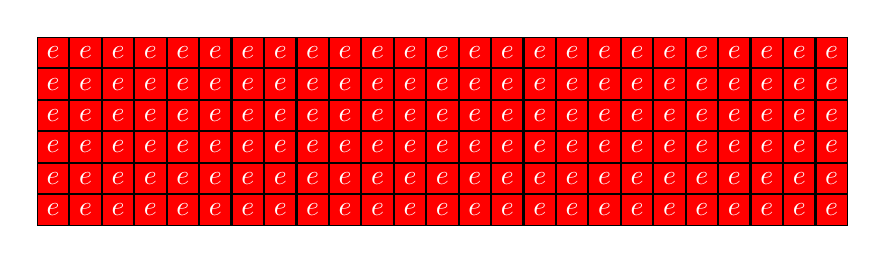
\begin{tikzpicture}[]
  \tikzstyle{every node}=[minimum size=3mm]
  \tikzset{pre/.style={draw,fill=black, text=white}}
  \let\mymatrixcontent\empty
  \foreach \i in {0,...,\the\numexpr \imgheight -1} {%
      \foreach \y in {1,...,\imgwidth} {%
        \checkbitmap(\the\numexpr \i*\imgwidth + \y)%
        \if 0\cachedata
            \edef\x{
            \noexpand\gappto\noexpand\mymatrixcontent{ \noexpand\node[pre, fill=black, text=black]{0}; \&}}\x
        \else
            \if 1\cachedata
                \edef\x{
                \noexpand\gappto\noexpand\mymatrixcontent{ \noexpand\node[pre, fill=white]{0}; \&}}\x
            \else
                \if 2\cachedata
                    \edef\x{
                    \noexpand\gappto\noexpand\mymatrixcontent{ \noexpand\node[pre, fill=blue]{2}; \&}}\x
                \else
                    \edef\x{
                    \noexpand\gappto\noexpand\mymatrixcontent{ \noexpand\node[pre, fill=red]{e}; \&}}\x
                \fi
            \fi
        \fi
      }
      \gappto\mymatrixcontent{\\}%
  }

  \matrix[matrix of math nodes,%
      nodes = {pre},%
      ampersand replacement=\&] {%
    \mymatrixcontent
  };
\end{tikzpicture}

\end{document}
